% LaTeX mintafájl szakdolgozat és diplomamunkáknak az
% SZTE Informatikai Tanszekcsoportja által megkövetelt
% formai követelményeinek megvalósításához
% Modositva: 2011.04.28 Nemeth L. Zoltan
% A fájl használatához szükséges a magyar.ldf 2005/05/12 v1.5-ös vagy későbbi verziója
% ez letölthető a http://www.math.bme.hu/latex/ weblapról, a magyar nyelvű szedéshez
% Hasznos információk, linekek, LaTeX leirasok a www.latex.lap.hu weboldalon vannak.
%


\documentclass[12pt]{report}



%Az ékezetes betűk használatához:
\usepackage[T1]{fontenc}% ékezetes szavak automatikus elválasztásához
\usepackage[utf8]{inputenc}% ékezetes szavak beviteléhez

%Magyar nyelvi támogatás (Babel 3.7 vagy későbbi kell!)
\def\magyarOptions{defaults=hu-min}
\usepackage[magyar]{babel}

% A formai kovetelmenyekben megkövetelt Times betűtípus hasznalata:
\usepackage{times}

%Az AMS csomagjai
\usepackage{amsmath}
\usepackage{amssymb}
\usepackage{amsthm}

%A fejléc láblécek kialakításához:
\usepackage{fancyhdr}

%Természetesen további csomagok is használhatók,
%például ábrák beillesztéséhez a graphix és a psfrag,
%ha nincs rájuk szükség természetesen kihagyhatók.
\usepackage{graphicx}
\usepackage{psfrag}

%Tételszerű környezetek definiálhatók, ezek most fejezetenkent egyutt szamozodnak, pl.
\newtheorem{tet}{Tétel}[chapter]
\newtheorem{defi}[tet]{Definíció}
\newtheorem{lemma}[tet]{Lemma}
\newtheorem{áll}[tet]{Állítás}
\newtheorem{köv}[tet]{Következmény}

%Ha a megjegyzések és a példak szövegét nem akarjuk dőlten szedni, akkor
%az alábbi parancs után kell őket definiální:
\theoremstyle{definition}
\newtheorem{megj}[tet]{Megjegyzés}
\newtheorem{pld}[tet]{Példa}

%Margók:
\hoffset -1in
\voffset -1in
\oddsidemargin 35mm
\textwidth 150mm
\topmargin 15mm
\headheight 10mm
\headsep 5mm
\textheight 237mm




\begin{document}

%% LaTeX fájl az elsõ kötéstábala látványterve
% SZTE Informatikai Tanszekcsoportja által megkövetelt
% formai követelményeinek megvalósításához
% A fájl használatához szükséges a magyar.ldf 1.5-ös vagy késõbbi verziója
% ez letölthetõ a http://www.math.bme.hu/latex/ weblapról, a magyar nyelvû szedéshez
% további hasznos információk és programok is vannak ott.
%

\documentclass[12pt]{report}

%Az ékezetes betûk használatához:
\usepackage{t1enc}
\usepackage[utf8]{inputenc}
% A megkövetelt Times betûtípus:
\usepackage{times}

%Magyar nyelvi támogatás (Babel 3.7 vagy késõbbi kell!)
\usepackage[magyar]{babel}

%Margók:
\hoffset -1in \voffset -1in \oddsidemargin 30mm \textwidth 150mm
\topmargin 15mm \headheight 10mm \headsep 5mm \textheight 237mm




\begin{document}


%A címoldalra se fej- se lábléc nem kell:
\thispagestyle{empty}
%Első kötéstábla:

\begin{center}
{\Large\bf Szegedi Tudományegyetem}

\vspace{0.5cm}

{\Large\bf Informatikai Intézet}

\vspace*{8.5cm}


{\Huge\bf SZAKDOLGOZAT}
%avagy {\Huge\bf DIPLOMAMUNKA}


\vspace*{7cm}

{\LARGE\bf Vas Laura}

\vspace*{0.6cm}

{\Large\bf 2021}

\end{center}

\end{document}


%A FEJEZETEK KEZDŐOLDALAINAK FEJ ES LÁBLÉCE:
%a plain oldalstílust kell átdefiniálni, hogy ott ne legyen fejléc:
\fancypagestyle{plain}{%
%ez mindent töröl:
\fancyhf{}
% a láblécbe jobboldalra kerüljön az oldalszám:
\fancyfoot[R]{\thepage}
%elválasztó vonal sem kell:
\renewcommand{\headrulewidth}{0pt}
}

%A TÖBBI OLDAL FEJ ÉS LÁBLÉCE:
\pagestyle{fancy}
\fancyhf{}
\fancyhead[L]{Recipe hoarder webes alkalmazás}
\fancyfoot[R]{\thepage}


%A címoldalra se fej- se lábléc nem kell:
\thispagestyle{empty}

\begin{center}
\vspace*{1cm}
{\Large\bf Szegedi Tudományegyetem}

\vspace{0.5cm}

{\Large\bf Informatikai Intézet}

\vspace*{3.8cm}


{\LARGE\bf Recipe hoarder webes alkalmazás}
\\\vspace*{0.3cm}
{\Large\bf (Recipe hoarder web application)}


\vspace*{3.6cm}

{\Large Szakdolgozat}
% vagy {\Large Szakdolgozat}

\vspace*{4cm}

%Értelemszerűen megváltoztatandó:
{\large
\begin{tabular}{c@{\hspace{4cm}}c}
\emph{Készítette:}     &\emph{Témavezető:}\\
\bf{Vas Laura}  &\bf{Dr. Bilicki Vilmos}\\
gazdaságinformatika szakos     &egyetemi adjunktus\\
hallgató&
\end{tabular}
}

\vspace*{2.3cm}

{\Large
Szeged
\\
\vspace{2mm}
2021
}
\end{center}


%A tartalomjegyzék:
\tableofcontents

%A \chapter* parancs nem ad a fejezetnek sorszámot
\chapter*{Feladatkiírás}
%A tartalomjegyzékben mégis szerepeltetni kell, mint szakasz(section) szerepeljen:
\addcontentsline{toc}{section}{Feladatkiírás}

A szakdolgozat során egy Angular keretrendszerben kialakított webes alkalmazás létrehozása volt a feladatom.
A projekt a Firebase-t használja adatbázisként. A fejlesztés során a legfőbb cél a recept importálás más honlapokról volt.
Az importálás második legfontosabb lépése az alapanyagok szétválogatása,
hogy később a bevásárlólistába helyezésnél a megyegyező anyagok összeadódjanak.

\chapter*{Tartalmi összefoglaló}
\addcontentsline{toc}{section}{Tartalmi összefoglaló}

A szakdolgozat céljául kitűzött témám egy Angular-ban írt web applikáció,
ami recept megjelenítésre és importálásra használható. Az importálás funkció lehetővé teszi,
hogy a felhasználók egy helyen gyűjsék a receptjeiket. Továbbá a regeptek összetevőit egy bevásárló listába ki tuják menteni,
ezzel is megkönnyítve a mindennapi életet.
A felhasználók a többiek álltal létrehozott receptek között tudnak keresni,
és a nekik tetsző recepteket ki tudják menteni a saját recetgyűjteményükbe.

Az applikáció egy weblap formályában lett megvalósítva, mivel így lehet a legtöbb ezközt elérni egyetlen kódbázissal.
A megvalósításhoz a már említett Angular keretrendszert használtam, illetve a Firebase felhő alapú szolgáltatásait.
Mivel mind a kettő (Angular, Firebase) a Google terméke, ezért várhatóan hosszútávon támogatva lesznek.

A felhasználó a recept URL-je alapján tud, recepet importálni, vagy manuálisan is tud létrehozni újjat. %TODO: ú/u j/jj?
Ekkor az importáláshoz egy szerver oldali funkció fut le és próbálja értelmezni a megkapott URL-en lévő html fájlt.
Ennek egy fontos lépése az, hogy az alapanyagok nevét, mértékegységét és mennyiségét az eredeti szövegből kiolvassa.
Ehhez regex-et illetve egy kölső konyvtárat használtam, ami sok mértékegység között tud átválltani.
Miután a receptet sikeresen importáltuk, azokat a Firebase FireStore adatbázisában tároljuk.

Mind az importálás mind az egész projekt során törekedtem, hogy minnél modulárisabb legyen a felépítés. 
A webapp fejlesztése során a PWA-t alkalmazva elérhető, hogy bizonyos funkciók offline is működjenek. 
A modern, könnyen kezelhető weblap számítógépen és telefonon egyaránt használható.

Kulcsszavak: Angular, Firebase, pipeline architektúra, PWA, telefonos nézet

%Bevezetés
\chapter*{Motiváció}
\addcontentsline{toc}{section}{Motiváció}

Egyetemisták, mint én is egyre közelebb vagyunk ahhoz az életformához, ahol önellátók vagyunk, ennek fontos része a főzés és étkezés. Manapság nagyon egyszerű különböző recepteket, különböző országokból, kultúrákból találni, viszont ez temérdeknyi weblapot jelenthet. Ennek hátulütője, hogy egy idő után követhetetlen lesz, hogy egyáltalán hova regisztráltunk, valamint, hogy “melyik weblapon is volt az a bizonyos recept, amit egyszer már kipróbáltam, és tetszett”. Személyes tapasztalatom ezzel kapcsolatba pedig, hogy én egy TXT fájlba mentegettem az URL címeket, hogy legközelebb is megtaláljam, de már kezdett nagyon követhetetlen lenni.

Azért választottam ezt az ötletet a szakdolgozatom témájának, mert ez egy személyes problémám már hosszú ideje és láttam már korábban próbálkozásokat, de egyik sem volt az én elképzelésemnek megfelelő. A célom az volt, hogy egy egyszerű URL cím másolással pillanatok alatt egy helyen lehessen a megtalálni mindent. 

A továbbiakban részletesen részletezem az általam tervezett és megvalósított webes applikáció felépítését és funkcióit. A bemutatót a konkurencia ismertetésével kezdem.




\chapter{Piacfelmérés}

Már létező programokra öt példát hoztam, amik mind valamilyen szinten különböznek.
Felhasználó körük, funkcióik, előnyök és hátrányok az én tervemhez képest.

\section{Grocy}
A Grocy egy lokálisan hostolható weblap. Irgalmatlanul részletes és rengeteg funkciója van, amihez, ha az ember hozzászokik és elég időt és törődést fektet bele, akkor egy nagyon hasznos program. Ellenben, mivel lokálisan van felépítve, ezért, ha valaki most kezdené el először használni, akkor nagyon sokáig tart, amíg igazán használható lehet. 

A recept kezelő lapja csak manuálisan feltölthető, tehát nincs importálásra lehetőség. Rendelkezik bevásárlólista és “sufni” opciókkal is. Az otthon lévő alapanyagokat egyessével, tetsző részletességgel fel lehet venni a “sufniba”, ezzel leltározva, hogy milyen alapanyagok vannak otthon. Ezekről eltárolható adatok közé tartozik, hogy mennyi van belőle, meddig jók, képet, de akár a vonalkódját is. A bevásárló lista pedig egyértelműen a vásárlást segítő funkció, aminek a végén, egy kattintásra átrakható “sufniba”. 

Már ezen kis leírás alapján is látszik, hogy ahhoz, hogy ez a rendszer használható legyen, egy komoly lokális adatbázist kell létrehozni az alapanyagokból és azok adatairól, valamint a receptekről. Ez a rendszer csak limitált tudású emberek számára használható, mivel már csak a telepítése is kicsit bonyolultabb, ezért átlag emberek számára nem ajánlott.

\section{Delish}
Tényleg, itt valóban vége.

\section{Yummly}
Tényleg, itt valóban vége.

\section{BigOven}
Tényleg, itt valóban vége.

\section{ChefTap}
Tényleg, itt valóban vége.


\chapter{Hosszú}
\section{Részletek}
Ebbe a fejezetbe pedig írunk sok sok szöveget. Szöveg, szöveg, szöveg,  szöveg, szöveg, szöveg,   szöveg, szöveg, szöveg
szöveg, szöveg, szöveg,  szöveg, szöveg, szöveg, szöveg, szöveg, szöveg, szöveg, szöveg, szöveg, szöveg, szöveg, szöveg,
szöveg, szöveg, szöveg, szöveg, szöveg, szöveg, szöveg, szöveg, szöveg, szöveg, szöveg, szöveg, szöveg, szöveg, szöveg,
szöveg, szöveg, szöveg, szöveg, szöveg, szöveg, szöveg, szöveg, szöveg, szöveg, szöveg, szöveg,
szöveg, szöveg, szöveg, szöveg, szöveg, szöveg, szöveg, szöveg, szöveg, szöveg, szöveg, szöveg, szöveg, szöveg, szöveg,
szöveg, szöveg, szöveg, szöveg, szöveg, szöveg, szöveg, szöveg, szöveg, szöveg, szöveg, szöveg, szöveg, szöveg, szöveg,
szöveg, szöveg, szöveg, szöveg, szöveg, szöveg, szöveg, szöveg, szöveg, szöveg, szöveg, szöveg, szöveg, szöveg, szöveg,
szöveg, szöveg, szöveg, szöveg, szöveg, szöveg, szöveg, szöveg, szöveg, szöveg, szöveg, szöveg, szöveg, szöveg, szöveg,
szöveg, szöveg, szöveg, szöveg, szöveg, szöveg, szöveg, szöveg, szöveg, szöveg, szöveg, szöveg, szöveg, szöveg, szöveg,
szöveg, szöveg, szöveg, szöveg, szöveg, szöveg, szöveg, szöveg, szöveg, szöveg, szöveg, szöveg, szöveg, szöveg, szöveg,
szöveg, szöveg, szöveg, szöveg, szöveg, szöveg, szöveg, szöveg, szöveg, szöveg, szöveg, szöveg, szöveg, szöveg, szöveg,
szöveg, szöveg, szöveg,  szöveg, szöveg, szöveg, szöveg, szöveg, szöveg, szöveg, szöveg, szöveg, szöveg, szöveg, szöveg,
szöveg, szöveg, szöveg, szöveg, szöveg, szöveg, szöveg, szöveg, szöveg, szöveg, szöveg, szöveg, szöveg, szöveg, szöveg,
szöveg, szöveg, szöveg, szöveg, szöveg, szöveg, szöveg, szöveg, szöveg, szöveg, szöveg, szöveg,
szöveg, szöveg, szöveg, szöveg, szöveg, szöveg, szöveg, szöveg, szöveg, szöveg, szöveg, szöveg, szöveg, szöveg, szöveg,
szöveg, szöveg, szöveg, szöveg, szöveg, szöveg, szöveg, szöveg, szöveg, szöveg, szöveg, szöveg, szöveg, szöveg, szöveg,
szöveg, szöveg, szöveg, szöveg, szöveg, szöveg, szöveg, szöveg, szöveg, szöveg, szöveg, szöveg, szöveg, szöveg, szöveg,
szöveg, szöveg, szöveg, szöveg, szöveg, szöveg, szöveg, szöveg, szöveg, szöveg, szöveg, szöveg, szöveg, szöveg, szöveg,
szöveg, szöveg, szöveg, szöveg, szöveg, szöveg, szöveg, szöveg, szöveg, szöveg, szöveg, szöveg, szöveg, szöveg, szöveg,
szöveg, szöveg, szöveg, szöveg, szöveg, szöveg, szöveg, szöveg, szöveg, szöveg, szöveg, szöveg, szöveg, szöveg, szöveg,
szöveg, szöveg, szöveg, szöveg, szöveg, szöveg, szöveg, szöveg, szöveg, szöveg, szöveg, szöveg, szöveg, szöveg, szöveg,
szöveg, szöveg, szöveg,  szöveg, szöveg, szöveg, szöveg, szöveg, szöveg, szöveg, szöveg, szöveg, szöveg, szöveg, szöveg,
szöveg, szöveg, szöveg, szöveg, szöveg, szöveg, szöveg, szöveg, szöveg, szöveg, szöveg, szöveg, szöveg, szöveg, szöveg,
szöveg, szöveg, szöveg, szöveg, szöveg, szöveg, szöveg, szöveg, szöveg, szöveg, szöveg, szöveg,
szöveg, szöveg, szöveg, szöveg, szöveg, szöveg, szöveg, szöveg, szöveg, szöveg, szöveg, szöveg, szöveg, szöveg, szöveg,
szöveg, szöveg, szöveg, szöveg, szöveg, szöveg, szöveg, szöveg, szöveg, szöveg, szöveg, szöveg, szöveg, szöveg, szöveg,
szöveg, szöveg, szöveg, szöveg, szöveg, szöveg, szöveg, szöveg, szöveg, szöveg, szöveg, szöveg, szöveg, szöveg, szöveg,
szöveg, szöveg, szöveg, szöveg, szöveg, szöveg, szöveg, szöveg, szöveg, szöveg, szöveg, szöveg, szöveg, szöveg, szöveg,
szöveg, szöveg, szöveg, szöveg, szöveg, szöveg, szöveg, szöveg, szöveg, szöveg, szöveg, szöveg, szöveg, szöveg, szöveg,
szöveg, szöveg, szöveg, szöveg, szöveg, szöveg, szöveg, szöveg, szöveg, szöveg, szöveg, szöveg, szöveg, szöveg, szöveg,
szöveg, szöveg, szöveg, szöveg, szöveg, szöveg, szöveg, szöveg, szöveg, szöveg, szöveg, szöveg, szöveg, szöveg, szöveg,
szöveg, szöveg, szöveg,  szöveg, szöveg, szöveg, szöveg, szöveg, szöveg, szöveg, szöveg, szöveg, szöveg, szöveg, szöveg,
szöveg, szöveg, szöveg, szöveg, szöveg, szöveg, szöveg, szöveg, szöveg, szöveg, szöveg, szöveg, szöveg, szöveg, szöveg,
szöveg, szöveg, szöveg, szöveg, szöveg, szöveg, szöveg, szöveg, szöveg, szöveg, szöveg, szöveg,
szöveg, szöveg, szöveg, szöveg, szöveg, szöveg, szöveg, szöveg, szöveg, szöveg, szöveg, szöveg, szöveg, szöveg, szöveg,
szöveg, szöveg, szöveg, szöveg, szöveg, szöveg, szöveg, szöveg, szöveg, szöveg, szöveg, szöveg, szöveg, szöveg, szöveg,

\chapter{Egyebek}

\section{Környezetek}
\begin{tet}
\label{tet-alap}
Ez itt egy tétel.
\end{tet}

%A bizonyítás \begin{proof} és \end{proof} közé kerül:
\begin{proof}
Ez pedig a bizonyítása, melyben szerepel egy képlet:
\begin{equation}
\begin{split}
E^{\text{globális}} &= \text{tét}_1\cdot E_1^{\text{elemi}}+\text{tét}_2\cdot
E_2^{\text{elemi}}+\ldots+\text{tét}_n\cdot E_n^{elemi} \\
&=E^{\text{elemi}}\left(\text{tét}_1+\text{tét}_2+\ldots+\text{tét}_n\right)\\
&=E^{\text{elemi}}\cdot\text{össztét}
\end{split}
\end{equation}
A második egyenlőségnél azt használtunk ki, hogy ...

Ezzel a bizonyítást befejeztük.
\end{proof}

\begin{defi}
\label{def-pelda}
Ez egy definíció. Számozása a tételekkel együtt történik.
\end{defi}

\begin{áll}
A követekező négy állítás egymással ekvivalens:
\label{áll-ekvivalencia}
  \begin{itemize}
  \item[(i)] $M$ és $N$ gyengén ekvivalensek.
  \item[(ii)] Minden $n$
  nemnegatív egész számra $|L_{M}\cap \Sigma_{1}^{n}|=|L_{N}\cap \Sigma_{2}^{n}|$ teljesül.
  \item[(iii)] Minden $n$ nemnegatív egész szám esetén
   létezik
  $ \pi_{n}: L_{M}\cap \Sigma_{1}^{n} \rightarrow L_{N}\cap \Sigma_{2}^{n} $ kölcsönösen egyértelmű
  leképezés.
  \item[(iv)] Minden nemnegatív $n$-re $x A^{n} y^{T}=x' A'^{n} y'^{T}$.
  \end{itemize}
\end{áll}

\begin{köv}
  Ez pedig egy következmény.
\end{köv}

\begin{pld}
  Ez lesz a példa, ezt nem szedjük dőlten.
\end{pld}

\begin{megj}
  A fejezetet pedig egy megjegyzés zárja.
\end{megj}


\section{Listák}

Ez egy felsorolás:
\begin{itemize}
    \item első
    \item második
      \subitem első
      \subitem második
    \item harmadik
    \item[$\clubsuit$]  saját jel is alkalmazható
\end{itemize}
Ez pedig egy számozott lista:
\begin{enumerate}
            \item hétfő
            \item kedd
            \item szerda
\end{enumerate}

%Oldaltörést is alkalmazhatunk
\pagebreak


\section{Egy táblázat és egy ábra}

A táblázat itt következik.
\begin{table}[!h]\label{strategia}
\caption{Példa stratégiatáblára a Black Jack esetében}
\begin{center}
\begin{tabular}{l||r|r|r|r|r|r|r|r|r|r}
&ász&2&3&4&5&6&7&8&9&10\\
\hline\hline
21&n&n&n&n&n&n&n&n&n&n\\
20&n&n&n&n&n&n&n&n&n&n\\
19&n&n&n&n&n&n&n&n&n&n\\
18&n&n&n&n&n&n&n&n&n&n\\
17&n&n&n&n&n&n&n&n&n&n\\
16&h&n&n&n&n&n&h&h&b&b\\
15&h&n&n&n&n&n&h&h&h&b\\
14&h&n&n&n&n&n&h&h&h&b\\
13&h&n&n&n&n&n&h&h&h&h\\
12&h&n&n&n&n&n&h&h&h&h\\
11&h&D&D&D&D&D&D&D&D&h\\
\end{tabular}
\end{center}
\end{table}

Lássunk egy ábrát is!
\begin{figure}[!h]
\unitlength 8mm
\begin{center}
\begin{picture}(8,6)
\thicklines
\multiput(0,1)(0,1){2}{\line(1,0){5}}
\multiput(3,0)(1,0){2}{\line(0,1){6}}
\multiput(1,0)(1,0){2}{\line(0,1){1}}
\multiput(6,0)(1,0){2}{\line(0,1){5}}
\multiput(0,1)(1,0){3}{\line(0,1){1}}
\multiput(2,4)(3,0){3}{\line(0,1){1}}
\multiput(3,0)(0,3){3}{\line(1,0){1}}
\multiput(6,0)(0,1){4}{\line(1,0){1}}
\multiput(7,2)(0,1){2}{\line(1,0){1}}
\multiput(2,4)(0,1){2}{\line(1,0){6}}
\put(5,1){\line(0,1){1}}
\put(8,2){\line(0,1){1}}
\put(1,0){\line(1,0){1}}
\put(1,1){\makebox(1,1){\(\sphericalangle\)}}
\put(7,2){\makebox(1,1){\(\$\)}}
\end{picture}
\end{center}
\caption{\label{labirintus}Labirintus bejárása}
\end{figure}

%laptörés:
\newpage

Külön fájlban elkészített grafika beillesztését a \ref{abra-automata} ábra szemlélteti.
\begin{figure}[h]
\centering
%A psfrag csomag használatával a (encapsulated)postcript abra feliratait LaTeX koddal helyettesíthatjük:
\psfrag{a}[c][c]{$q_0$}
\psfrag{b}[c][c]{$q_1$}
\psfrag{c}[c][c]{$q_2$}
\psfrag{d}[c][c]{$q_3$}
\psfrag{e}[c][c]{$q_4$}
\psfrag{f}[c][c]{$q_5$}
\psfrag{g}[c][c]{$q_6$}
\psfrag{h}[c][c]{$q_7$}
\psfrag{0}[c][c]{$a_{0}$}
\psfrag{9}[c][c]{$a_{9}$}
\psfrag{3}[c][c]{$a_{3}$}
\psfrag{12}[c][c]{$a_{12}$}
\psfrag{15}[c][c]{$a_{15}$}
%Garfika belillesztese, "scale2 a nagyitas/kicinyites merteke, itt 80%.
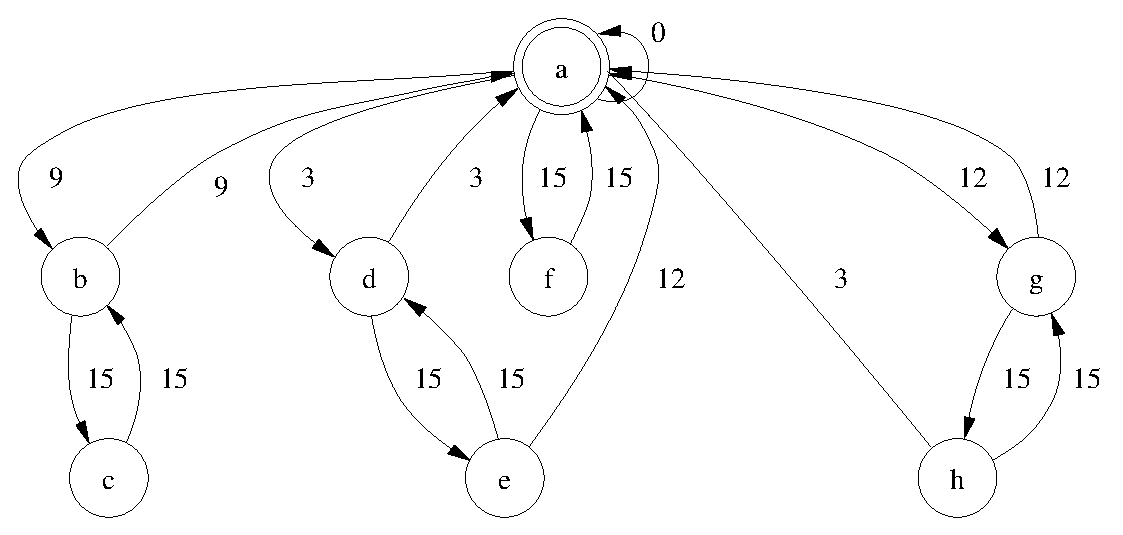
\includegraphics[scale=0.8]{abra.eps}
\caption{\label{abra-automata} A $4\times m$-es tábla lefedéseinek mátrixreprezentációit felismerő automata}
\end{figure}


\chapter{Függelék}

\section{A program forráskódja}
A függelékbe kerülhetnek a hosszú táblázatok, vagy mondjuk egy programlista:
% A verbatim kornyezet hasznalatanal ügyeljünk rá, hogy az editor a szóközöjket át ne írja tab karakterekre!
\begin{verbatim}
   while (ujkmodosito[i]<0)
   {
      if (ujkmodosito[i]+kegyenletes[i]<0)
      {
         j=i+1;
         while (j<14)
         if (kegyenletes[i]+ujkmodosito[j]>-1) break;
         else j++;
         temp=ujkmodosito[j];
         for (l=i;l<j;l++) ujkmodosito[l+1]=ujkmodosito[l];
         ujkmodosito[i]=temp;
      }
      i++;
   }
\end{verbatim}


\chapter*{Nyilatkozat}
%Egy üres sort adunk a tartalomjegyzékhez:
\addtocontents{toc}{\ }
\addcontentsline{toc}{section}{Nyilatkozat}
%\hspace{\parindent}

% A nyilatkozat szövege más titkos és nem titkos dolgozatok esetében.
% Csak az egyik tipusú myilatokzatnak kell a dolgozatban szerepelni
% A ponok helyére az adatok értelemszerűen behelyettesídendők es
% a szakdolgozat /diplomamunka szo megfeleloen kivalasztando.


%A nyilatkozat szövege TITKOSNAK NEM MINŐSÍTETT dolgozatban a következő:
%A pontokkal jelölt szövegrészek értelemszerűen a szövegszerkesztőben és
%nem kézzel helyettesítendők:

\noindent
Alulírott \makebox[4cm]{\dotfill} szakos hallgató, kijelentem, hogy a dolgozatomat a Szegedi Tudományegyetem, Informatikai Intézet \makebox[4cm]{\dotfill} Tanszékén készítettem, \makebox[4cm]{\dotfill} diploma megszerzése érdekében.

Kijelentem, hogy a dolgozatot más szakon korábban nem védtem meg, saját munkám eredménye, és csak a hivatkozott forrásokat (szakirodalom, eszközök, stb.) használtam fel.

Tudomásul veszem, hogy szakdolgozatomat / diplomamunkámat a Szegedi Tudományegyetem Informatikai Intézet könyvtárában, a helyben olvasható könyvek között helyezik el.

\vspace*{2cm}

\begin{tabular}{lc}
Szeged, \today\
\hspace{2cm} & \makebox[6cm]{\dotfill} \\
& aláírás \\
\end{tabular}


\vspace*{4cm}

%A nyilatkozat szövege TITKOSNAK MINŐSÍTETT dolgozatban a következő:

\noindent
Alulírott \makebox[4cm]{\dotfill} szakos hallgató, kijelentem, hogy a dolgozatomat a Szegedi Tudományegyetem, Informatikai Intézet \makebox[4cm]{\dotfill} Tanszékén készítettem, \makebox[4cm]{\dotfill} diploma megszerzése érdekében.

Kijelentem, hogy a dolgozatot más szakon korábban nem védtem meg, saját munkám eredménye, és csak a hivatkozott forrásokat (szakirodalom, eszközök, stb.) használtam fel.

Tudomásul veszem, hogy szakdolgozatomat / diplomamunkámat a TVSZ 4. sz. mellékletében leírtak szerint kezelik.

\vspace*{2cm}

\begin{tabular}{lc}
Szeged, \today\
\hspace{2cm} & \makebox[6cm]{\dotfill} \\
& aláírás \\
\end{tabular}





\chapter*{Köszönetnyilvánítás}
\addcontentsline{toc}{section}{Köszönetnyilvánítás}

Ezúton szeretnék köszönetet mondani \textbf{X. Y-nak} ezért és ezért \ldots


%% Az itrodalomjegyzek keszitheto a BibTeX segedprogrammal:
%\bibliography{diploma}
%\bibliographystyle{plain}

%VAGY "kézzel" a következő módon:

\begin{thebibliography}{9}
%10-nél kevesebb hivatkozás esetén

%\begin{thebibliography}{99}
% 10-nél több hivatkozás esetén

\addcontentsline{toc}{section}{Irodalomjegyzék}

%Elso szerzok vezetekneve alapjan ábécérendben rendezve.


%folyóirat cikk: szerzok(k), a folyóirat neve kiemelve,
%az evfolyam felkoveren, zarojelben az evszam, vegul az oldalszamok es pont.
\bibitem{Gischer}
J. L. Gischer,
The equational theory of pomsets.
\emph{Theoret. Comput. Sci.}, \textbf{61}(1988), 199--224.

%könyv (szerzo(k), a könyv neve kiemelve, utana a kiado, a kiado szekhelye, az evszam es pont.)
\bibitem{Pin}
J.-E. Pin,
\emph{Varieties of Formal Languages},
Plenum Publishing Corp., New York, 1986.





\end{thebibliography}




\end{document}
